\section*{\bfseries\large\MakeUppercase{Appendix A}} \label{A}

\topskip0pt
\vspace*{\fill}
\begin{center}
    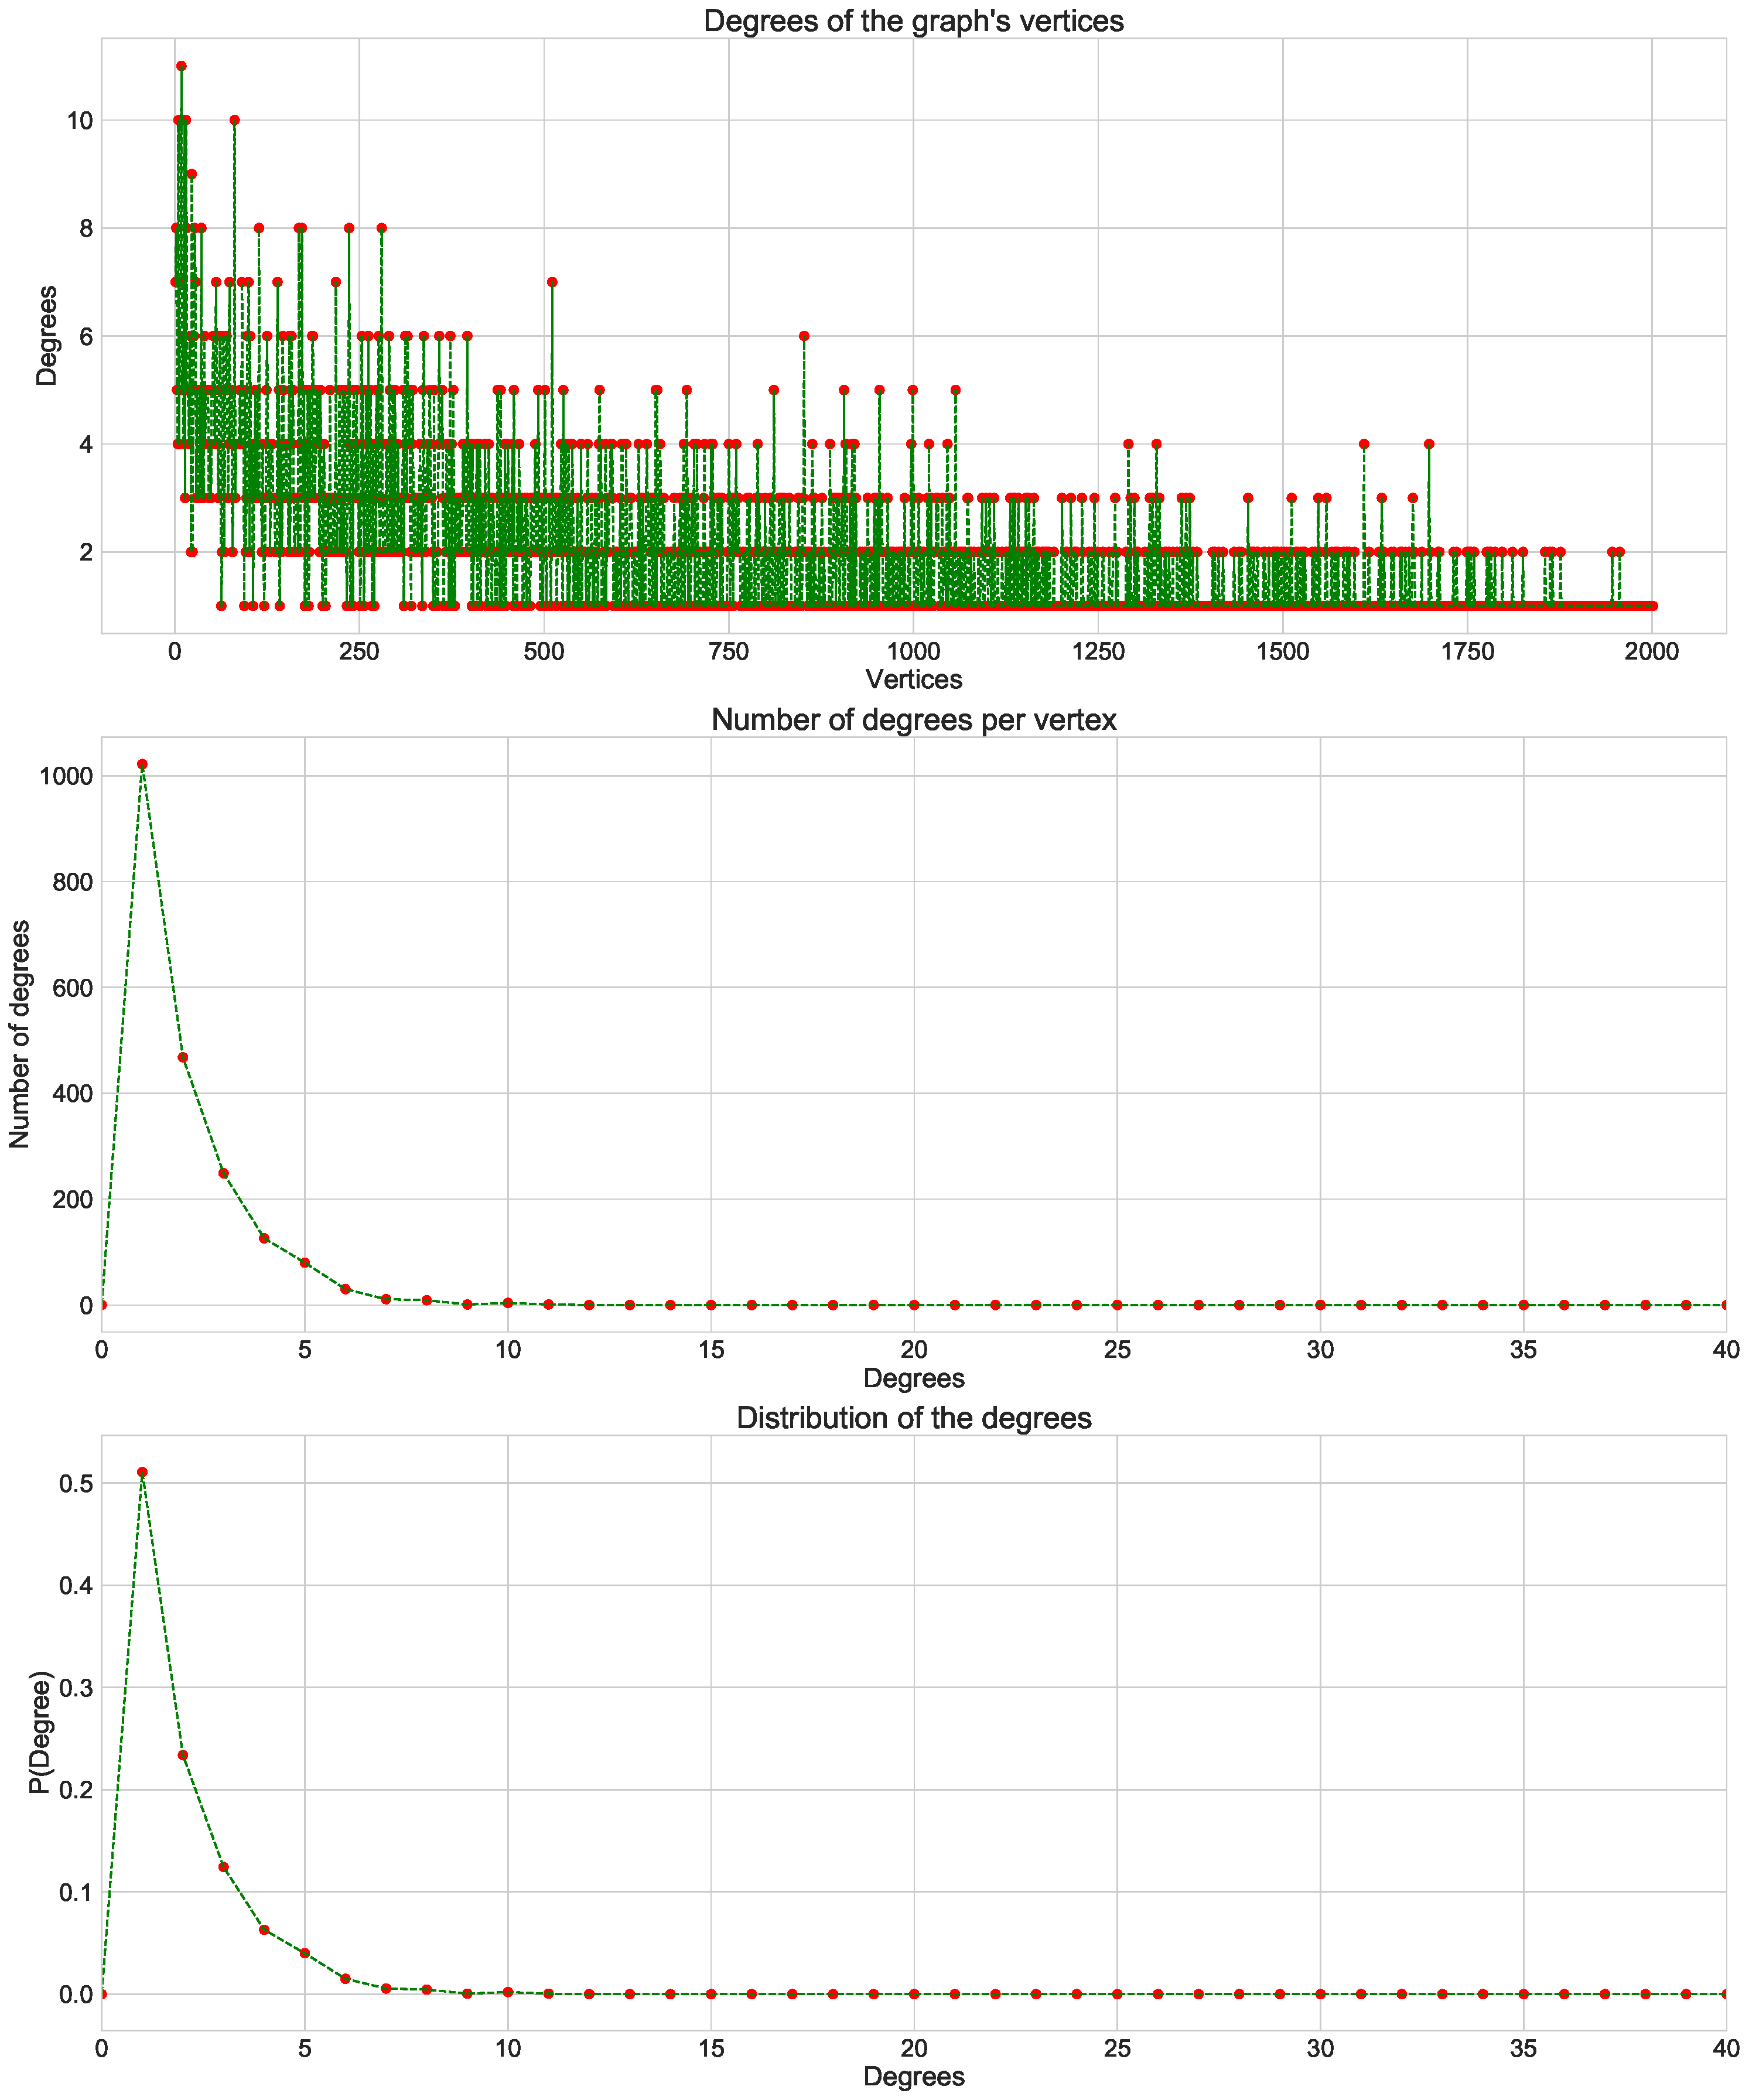
\includegraphics[width=0.9\textwidth]{images/pm_1.pdf}
    \captionof{figure}{A \pmd $E=100$ élre, 1. kezdőfeltétel\\Fent: Az egyes csúcsok fokszáma\\Középen: Adott fokszámú csúcsok darabszáma\\Lent: A csúcsok fokszámának eloszlása} \label{fig:1}
\end{center}
\vspace*{\fill}
\newpage
\topskip0pt
\vspace*{\fill}
\begin{center}
    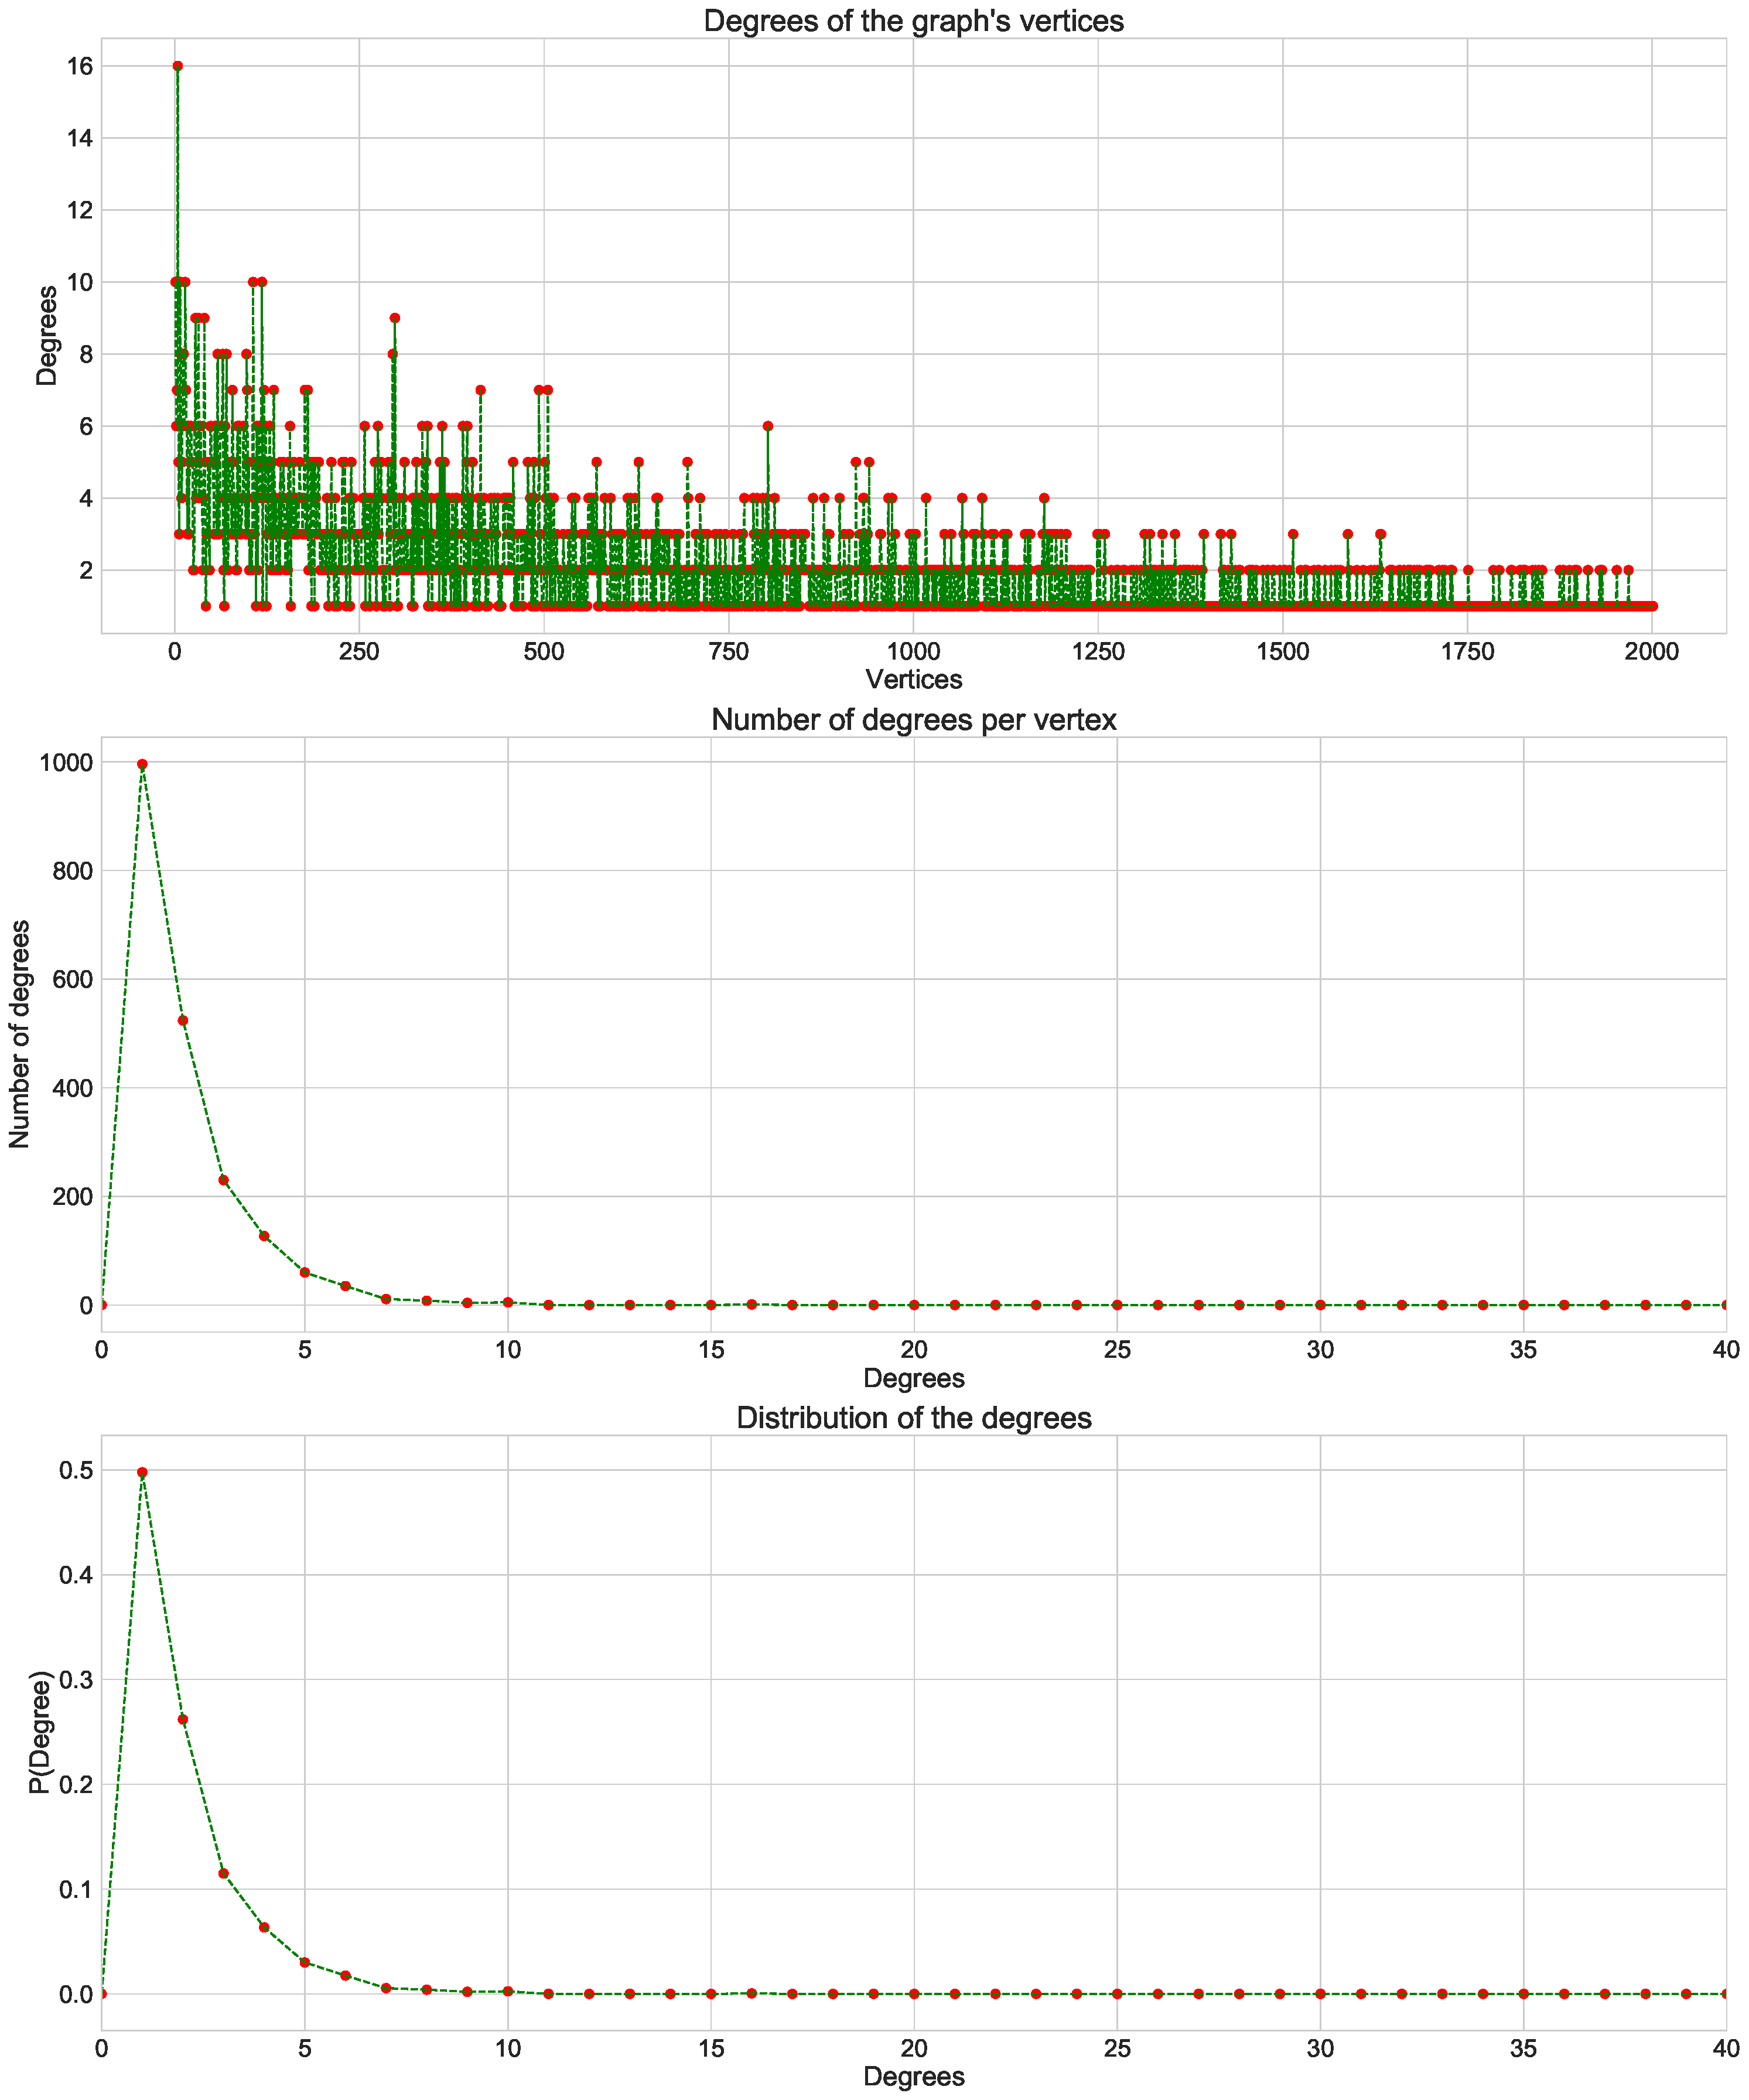
\includegraphics[width=0.95\textwidth]{images/pm_2.pdf}
    \captionof{figure}{A \pmd $E=100$ élre, 2. kezdőfeltétel\\Fent: Az egyes csúcsok fokszáma\\Középen: Adott fokszámú csúcsok darabszáma\\Lent: A csúcsok fokszámának eloszlása} \label{fig:2}
\end{center}
\vspace*{\fill}
\newpage
\topskip0pt
\vspace*{\fill}
\begin{center}
    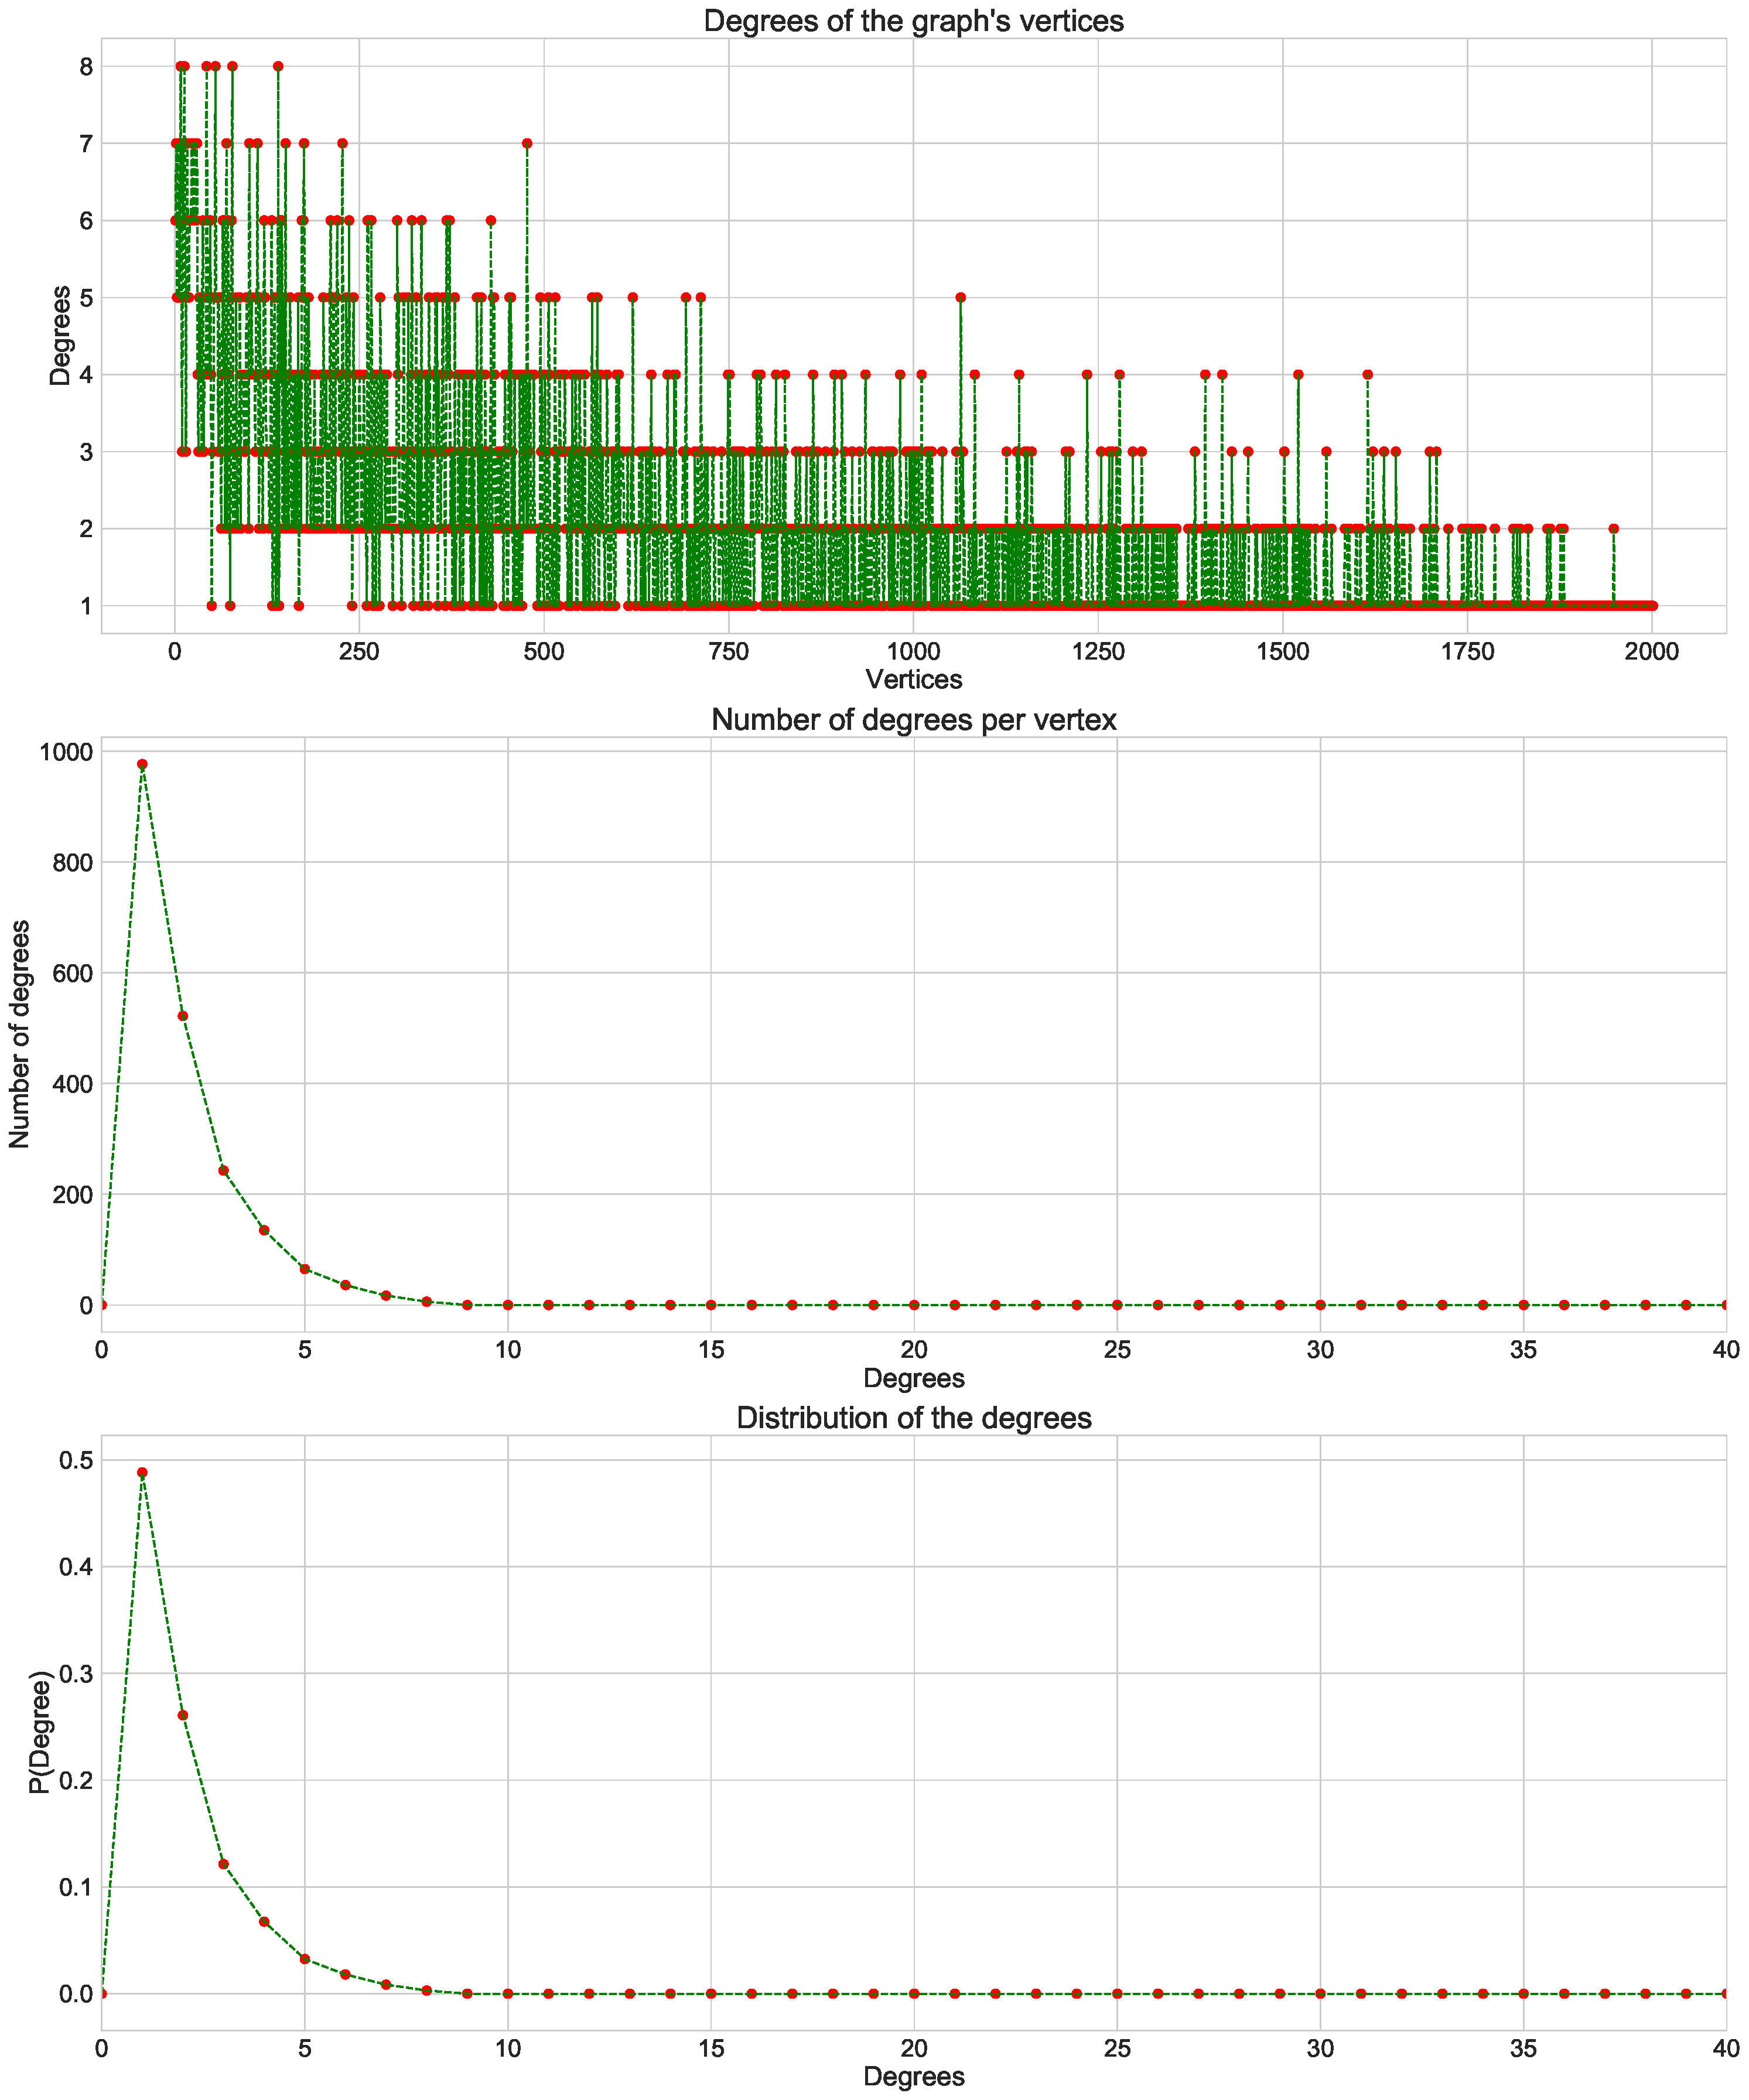
\includegraphics[width=0.95\textwidth]{images/pm_3.pdf}
    \captionof{figure}{A \pmd $E=100$ élre, 3. kezdőfeltétel\\Fent: Az egyes csúcsok fokszáma\\Középen: Adott fokszámú csúcsok darabszáma\\Lent: A csúcsok fokszámának eloszlása} \label{fig:3}
\end{center}
\vspace*{\fill}
\newpage
\topskip0pt
\vspace*{\fill}
\begin{center}
    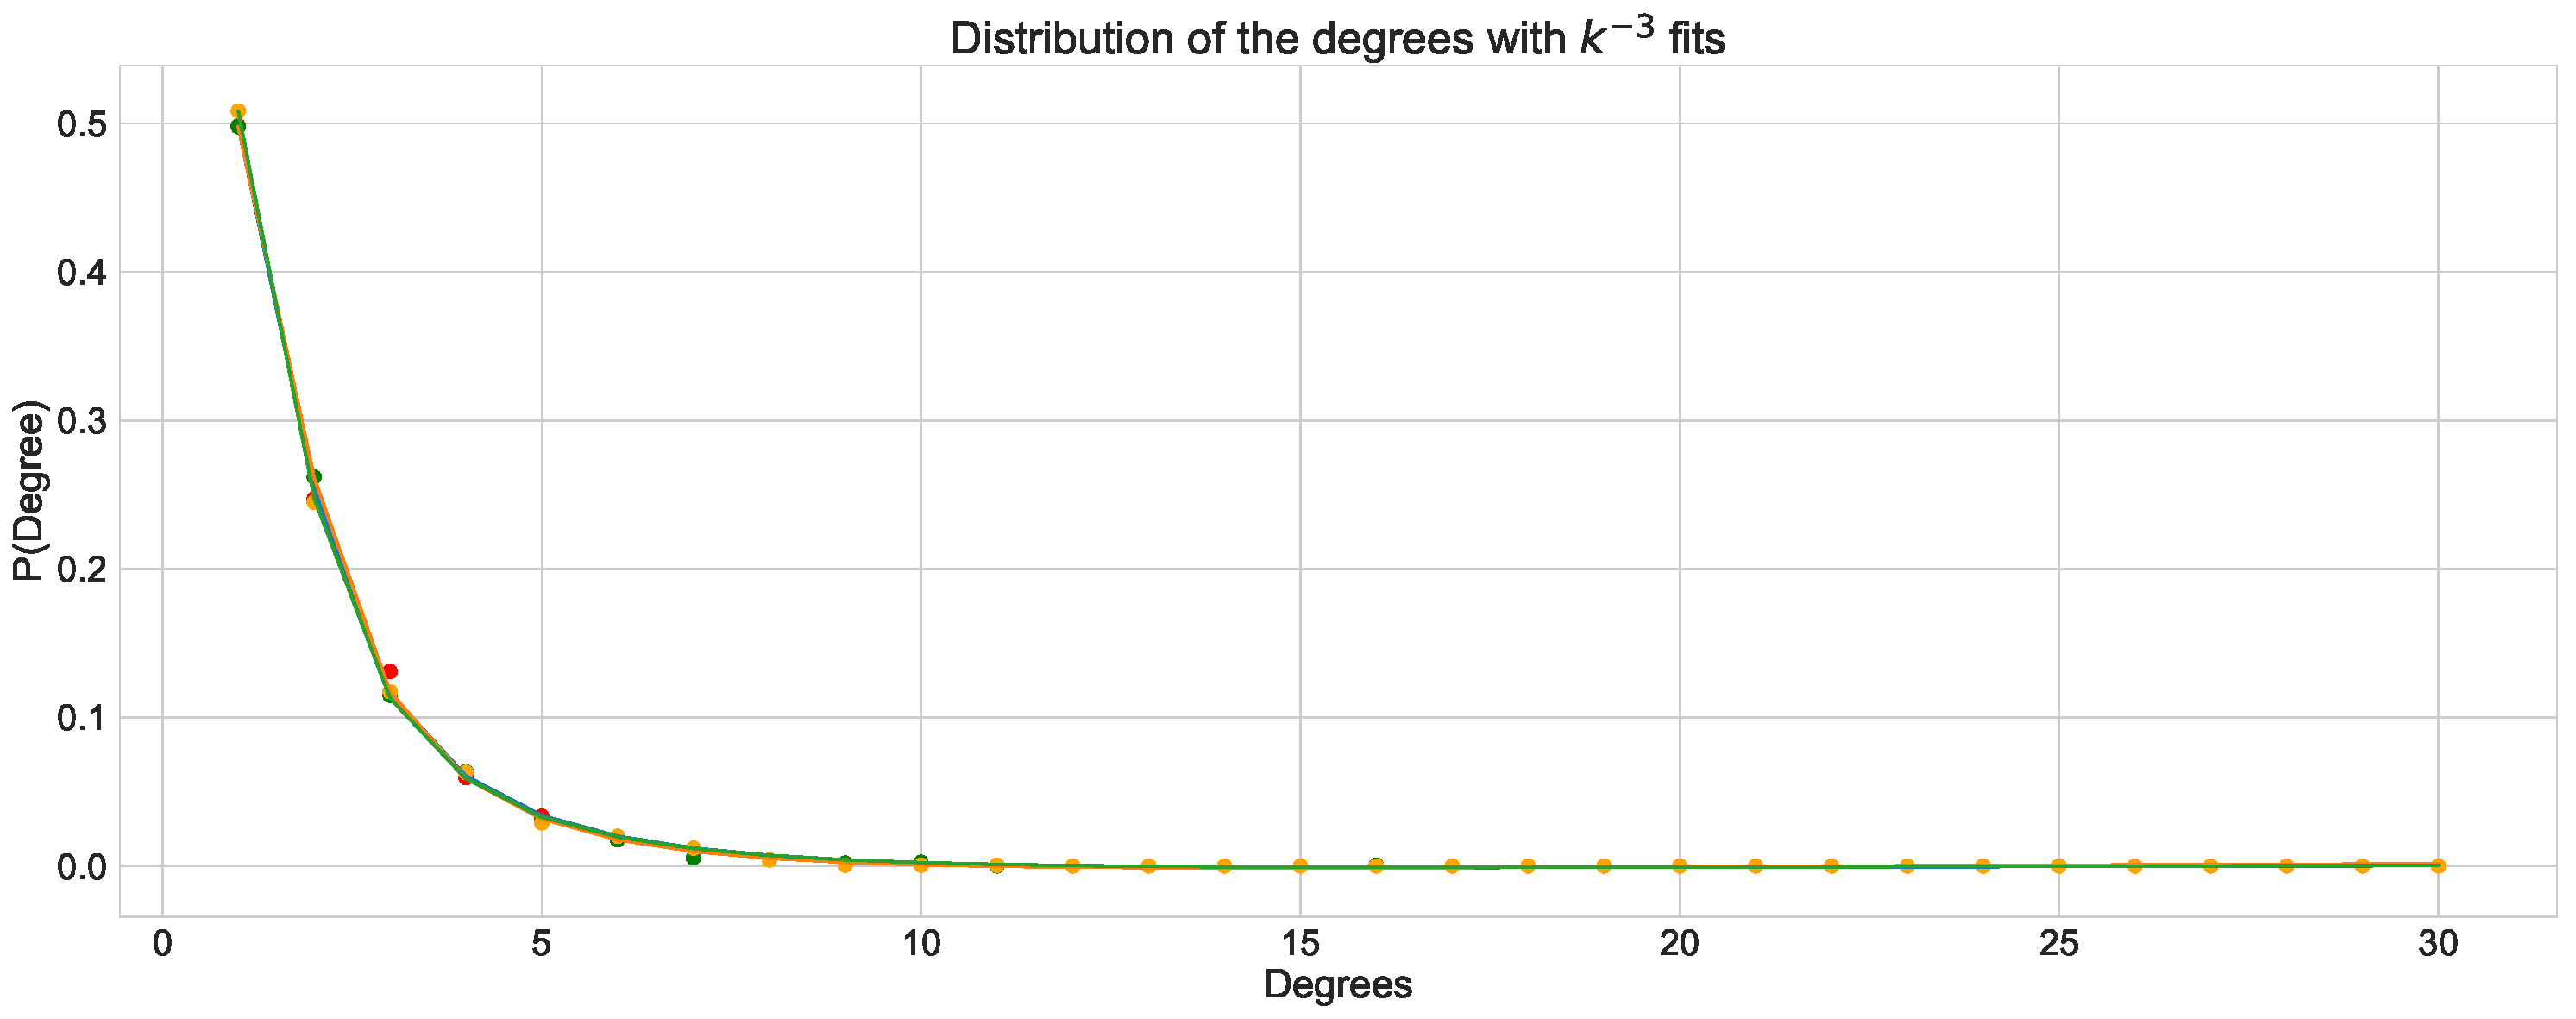
\includegraphics[width=\textwidth]{images/pm_diff.pdf}
    \captionof{figure}{A \pmd különböző $E$ élszámok esetére vett fokszámeloszlása, mindhárom kezdőfeltétel mellett.\\A képen látható pontok a szimulációban mért értékek, a görbék pedig a hozzájuk illesztett $k^{-3}$ polinomok.} \label{fig:4}
\end{center}
\begin{center}
    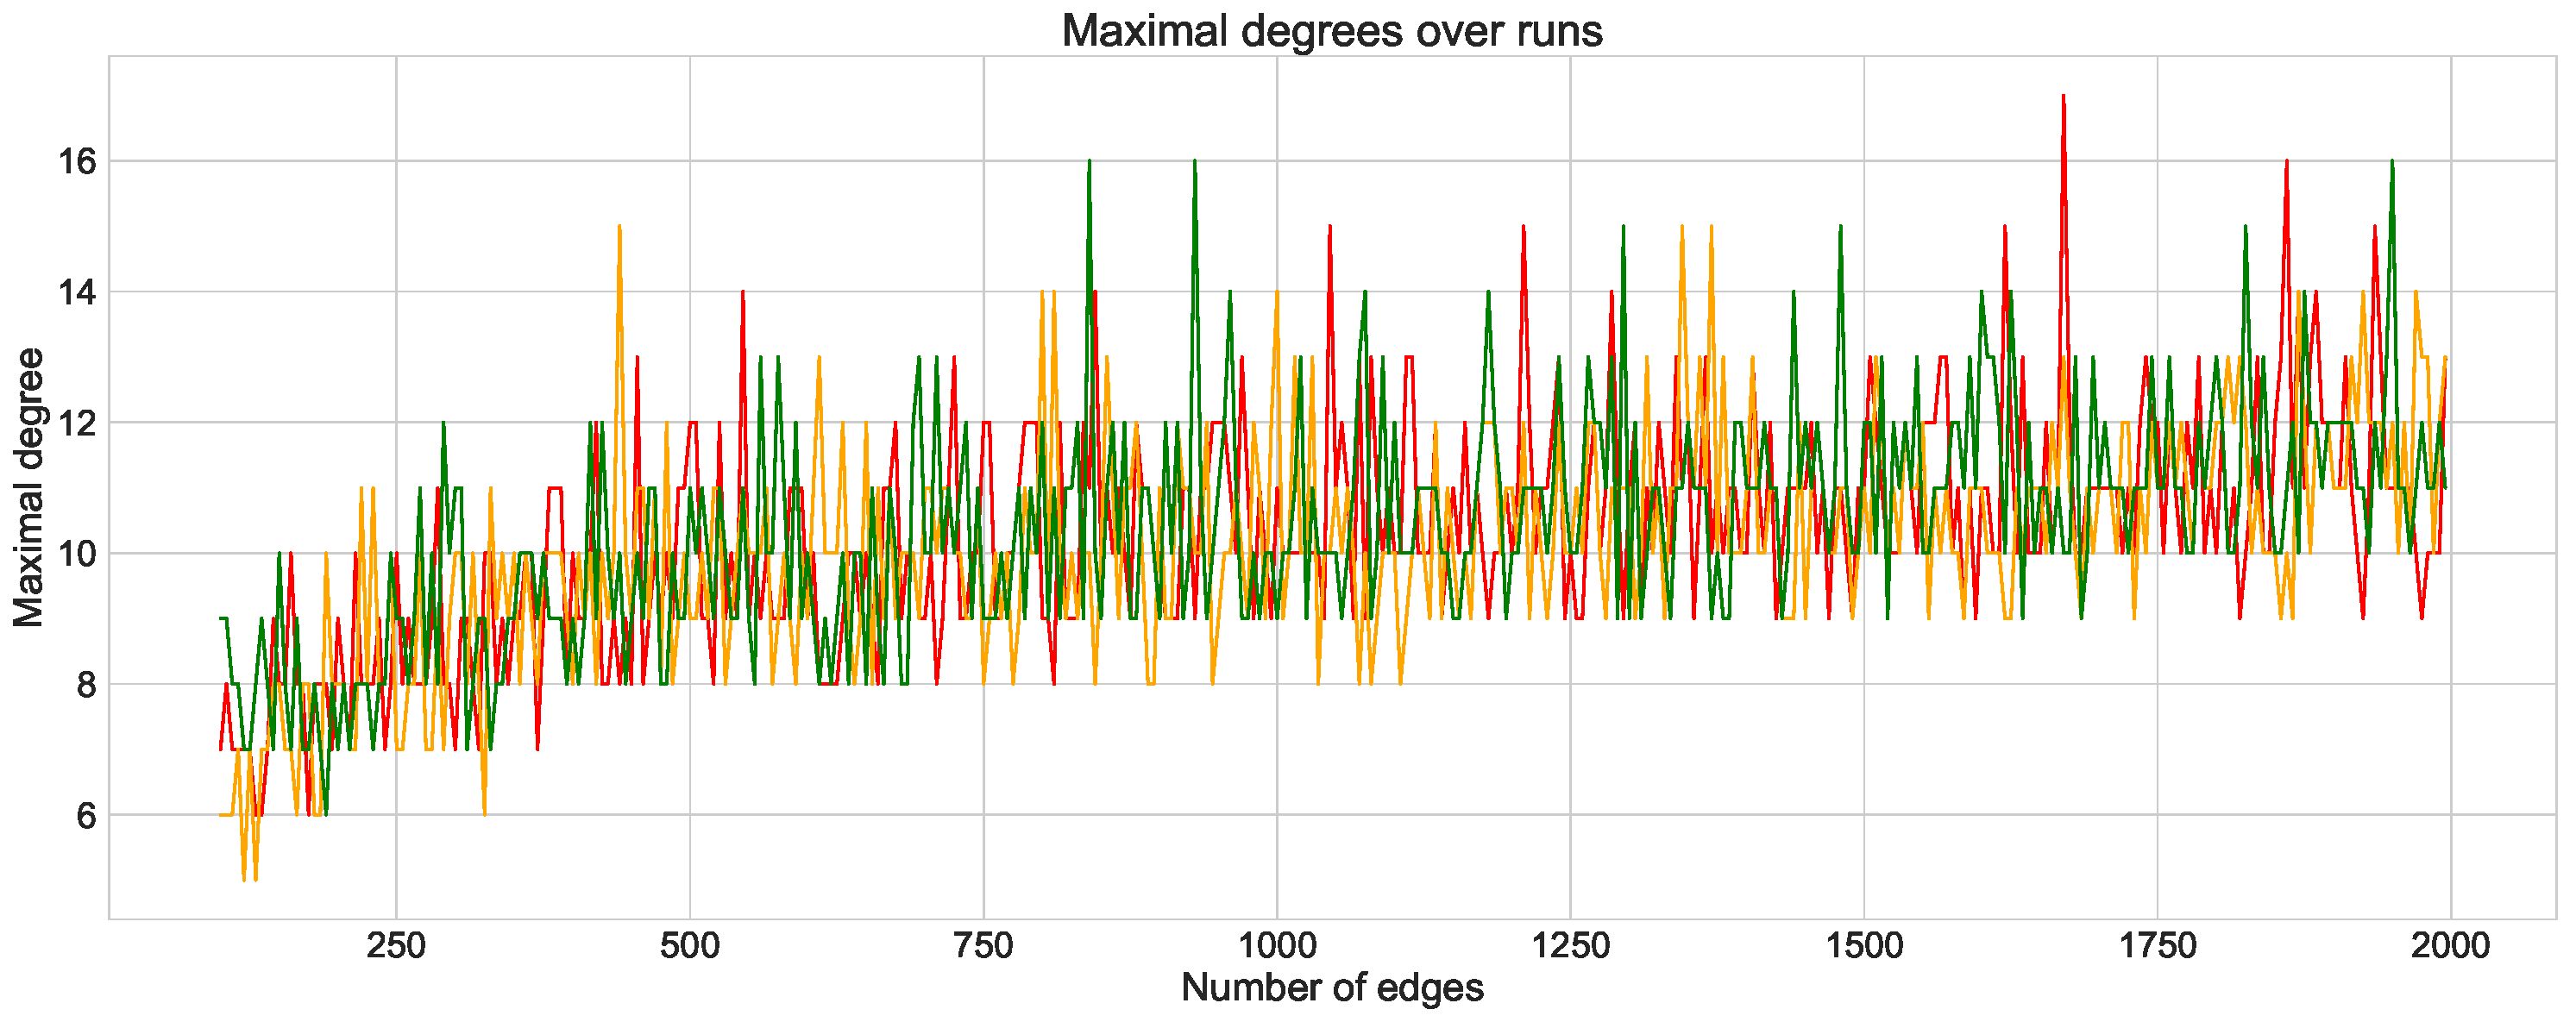
\includegraphics[width=\textwidth]{images/pm_maxdegrees.pdf}
    \captionof{figure}{A \pmd különböző $E$ élszámok esetén megjelenő maximális fokszáma.\\A szimuláció $E=100$ és $E=2000$ élszámértékek között futott.} \label{fig:5}
\end{center}
\vspace*{\fill}